\chapter{BPA数据读取与转换}

\section{BPA数据卡片的分类}

主要的数据卡片可分为四类,分别为区域控制、节点数据、支路数据及节点数据修改卡。

\begin{table}[h]
\centering
\begin{tabular}{ll}
\toprule
卡片分类 & 卡片描述\\
\midrule
 区域控制数据卡 & AC、A,指定参与区域功率交换的分区及安排交换功率量 \\ 
 & AO,按区域分类输出 \\ 
 & I,指定区域交换功率 \\ 
 \midrule
 节点数据卡 & B,交流节点卡\\
 & BD,两端直流节点卡\\
 & BM,多端直流节点卡\\
 & +,延续节点卡\\
 & X,可切换电抗、电容器卡\\
 \midrule
 支路数据卡 & L,对称线路卡\\
 & LD,两端直流线路卡\\
 & LM,多端直流线路卡\\
 & T,变压器和移相器卡\\
 & R,带负荷调压变压器调节数据卡\\
 & E,不对称等值支路卡\\
 & RZ,可快速调整的线路串补数据卡\\
 \midrule
 数据修改卡 & P,系统中发电出力和负荷按百分数修改卡\\
 & Z,分区重新命名卡\\
 & DZ,分区删除卡\\
\bottomrule
\end{tabular}
\caption{主要数据卡片分类}
\end{table}

在BPA到DIgSILENT的数据转换程序中,我们需要处理的主要是一下这些卡片:B,交流节点卡;L,对称线路卡;T,变压器和移相器卡;P,系统中发电出力和负荷按百分数修改卡。下面来详细介绍各个卡片的数据格式和模型。

\section{B卡}

\begin{figure}[H]
\centering
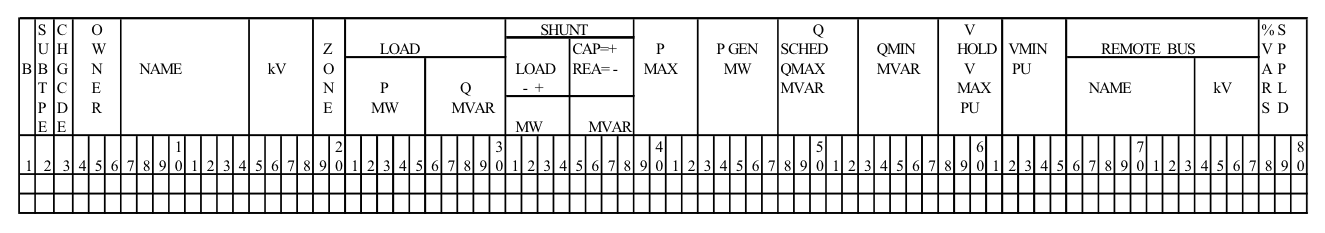
\includegraphics[width=1.05\textwidth]{images/Paper_Fig_17.png}
\setcaptionwidth{\linewidth}
\caption{B卡数据}
\end{figure}

\begin{spacing}{1.0}
\begin{longtable}[h]{llp{0.85\columnwidth}}
\toprule
列 & 格式 & 内容\\
 \midrule
1 & A1 & 卡片类型-B\\
 & A1 & 卡片子型-各子型如下: \\ 
 & & 空白-PQ节点\\ & &
T-PQ节点,但节点电压受带负荷调压变压器控制\\ & &
C-PQ节点,但节点电压受某发电机控制\\ & &
V-PQ节点,但节点电压有限制值:$V_{min}<V<V_{max}$,当电压越界
时,自动转换为PV节点,这时Q起变化,以保证电压在限制值
内,由此产生的未安排	无功,将由程序自动装上电容器(电抗
器)来平衡 \\ & &
E-PV节点,无功出力没有限制,但为达到控制电压,无功出力
超过上下限时,超过部分无功称为未安排无功,程序自动装上电
容器或电抗器 \\ & &
Q-PV节点,但节点无功功率有限制值:$Q_{min}<Q<Q_{max}$,当越界
时,自动转换为PQ节点 \\ & &
G-PV节点(其为发电机节点),缺省电压在0.95~1.15之间变
化,并去控制BC节点的电压。其无功Q也有限制,当Q越限时,中
止电压控制。被控节点不可以是Vθ节点、BG节点或者其它已处
于被控状态下的节点 \\ & &
F-在计算中先作为PV节点,待有功功率P收敛后再自动转换为B
(PQ)节点 \\ & &
S-Vθ节点,为交流同步网的缓冲机 \\ & &
J-在采用改进的牛顿-拉夫逊法时作为BS节点,当解法转化为牛
顿-拉夫逊法以后,该节点自动转换为B(PQ)节点 \\ & &
K-在采用改进的牛顿-拉夫逊法时作为BS节点,当解法转化为牛
顿-拉夫逊法以后,该节点自动转换为BE(PV)节点 \\ & &
L-在采用改进的牛顿-拉夫逊法时作为BS节点,当解法转为牛顿-
拉夫逊法以后,该节点自动转换为BQ(PV节点,$Q_{min}\leqslant Q\leqslant
Q_{max}$)节点 \\ & &
X-在该节点装有电抗器或者电容器,由程序自动控制投切电抗器
或者电容器,以维持该节点或者其它节点的电压为给定值。\\
 
\bottomrule
\end{longtable}
\end{spacing}

其中S节点的判断比较重要,需要特殊处理。需在同步电机卡中选定为reference machine,如图5.1所示。

\begin{figure}[H]
\centering
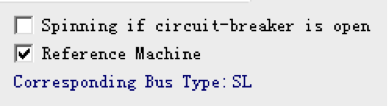
\includegraphics[width=0.6\textwidth]{images/Paper_Fig_18.png}
\setcaptionwidth{\linewidth}
\caption{reference machine选择}
\end{figure}

\subsection{DIgSILENT负载模型介绍及数据转换}

\begin{spacing}{1.0}
\begin{longtable}[h]{llp{0.8\columnwidth}}
\toprule
列 & 格式 & 内容\\
 \midrule
2 & A1 & 修改码,在程序中不做处理\\
4-6 & A3 & 所有者代码-用于确定区域功率交换中联络线的测点和输出表中按所有者分类的分析报告,可不填,当不填时在DIgSILENT中选取为0号owner。 \\ 
7-18 & A8, F4.0 & 节点名称(7-14),此节点名称直接设这为DIgSILENT节点ElmTerm项的NAME,而基准电压(kV)(15-18)则直接设定为DIgSILENT的Nominal Voltage(标准电压)。\\
19-20 & A2 & 节点所在的分区名称,在区域功率交换中用于确定区域的分区,在系统合并和按分区分类输出时也有用。在转换到DIgSILENT的过程中作为网络数据的大框架,使所有节点,线路,变压器等元器件都转换在这项之下。\\
\textbf{21-30} & \textbf{2F5.0} & \textbf{以MW和Mvar表示的恒定负荷,无功正值为感性、负值为容性。这两项数据正是该节点负载的数据信息。}\\
\bottomrule
\end{longtable}
\end{spacing}

如上表所示,第21-30列为描述恒定负荷所需要的有功、无功信息,在DIgSILENT中对应的是负载模型。

\begin{figure}[H]
\centering
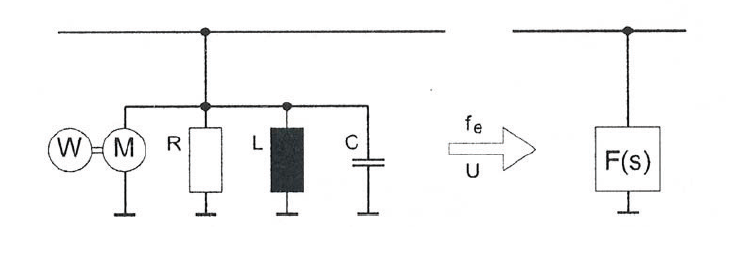
\includegraphics[width=1.0\textwidth]{images/Paper_Fig_19.png}
\setcaptionwidth{\linewidth}
\caption{DIgSILENT普通负载模型}
\end{figure}

DIgSILENT中采用的负荷模型是一种动态负荷、静态负荷与用户自定义“特殊”负荷的综合,在DIgSILENT中负载模型描述如图5.3.

通常情况下选择为3项平衡负载,切数据输入模式(Input Mode)选择为Default模式。在平衡负载情况之下,负载的潮流分析可不用专门将其专门设为单相或双相负载。其潮流模型如下:

\begin{figure}[H]
\centering
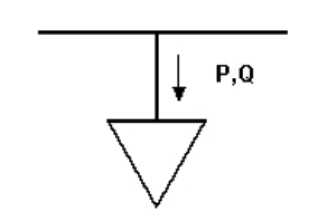
\includegraphics[width=0.4\textwidth]{images/Paper_Fig_20.png}
\setcaptionwidth{\linewidth}
\caption{DIgSILENT平衡负载的潮流模型}
\end{figure}

负荷电压依赖性可以如下述方程建模:
$$P = P_0\left[aP*(\frac{v}{v_0})^{e\_ap} + bP*(\frac{v}{v_0})^{e\_bp} + cP*(\frac{v}{v_0})^{e\_cp}\right] \eqno{(5.1)}$$
其中
$$1 - aP - bP = cP \eqno{(5.2)}$$
$$Q = Q_0\left[aP*(\frac{v}Q{v_0})^{e\_aQ} + bQ*(\frac{v}{v_0})^{e\_bQ} + cQ*(\frac{v}{v_0})^{e\_cQ}\right] \eqno{(5.3)}$$
其中
$$1 - aQ - bQ = cQ \eqno{(5.4)}$$

\begin{center}
\begin{table}[h]
\centering
\begin{tabular}{p{0.2\columnwidth}p{0.2\columnwidth}}
\toprule
指数 & 常量\\
\midrule
 0 & 功率\\
 1 & 电流\\
 2 & 电阻\\
\bottomrule
\end{tabular}
\caption{为实现不同负载功效的指数选取}
\end{table}
\end{center}


通过对上述公式的几项指数经行赋值,就可以对固有的负载建模。表5.4提供了分别实现恒功率,恒电流以及恒定电阻特性的负载模型所需要的指数参数。但是相应的每个系数($aP, bP, cP, aQ, bQ, cQ$)则可以任意定义如图:

\begin{figure}[H]
\centering
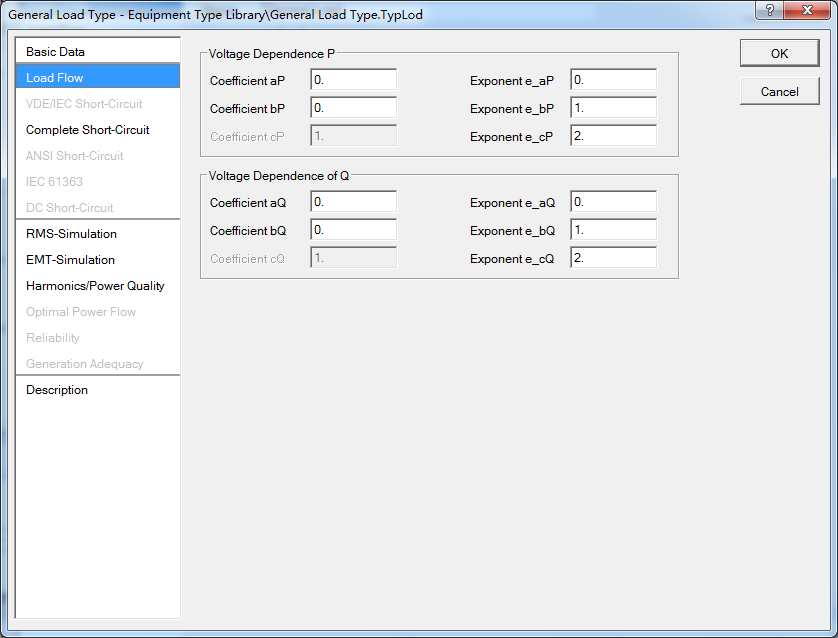
\includegraphics[width=0.9\textwidth]{images/Paper_Fig_21.png}
\setcaptionwidth{\linewidth}
\caption{不同功能负载实现的系数表格图}
\end{figure}

如图5.5所示,以有功功率为例,图中的参数使得有功负载的最后方程形式为$P = P_0\left[aP*(\frac{v}{v_0})^0 + bP*(\frac{v}{v_0})^1 + cP*(\frac{v}{v_0})^2\right]$,可见负载有功不仅与恒定功率$P_0$有关,还与负载电压平方有关,而且负载功率受电压控制,这正好与$P = \frac{U^2}{R}$公式一致,所以当取$aP = bP = aQ = bQ = 0$,$cP = cQ = 1$时可以表示为一恒阻抗负荷,即可以作为一个阻抗使用。

同理,当取$aP = aQ = 1$,$bP = bQ = 0$,$cP = cQ = 0$时,则是恒功率负载。

通过负荷调节因子,负载可以单独被放大或者缩小如下:

$$P = scale * P_0 \eqno{(5.5)}$$
$$Q = scale * Q_0 \eqno{(5.6)}$$
$$P = scale * P_0\left[aP*(\frac{v}{v_0})^{e\_ap} + bP*(\frac{v}{v_0})^{e\_bp} + cP*(\frac{v}{v_0})^{e\_cp}\right] \eqno{(5.7)}$$
$$Q = scale * Q_0\left[aP*(\frac{v}Q{v_0})^{e\_aQ} + bQ*(\frac{v}{v_0})^{e\_bQ} + cQ*(\frac{v}{v_0})^{e\_cQ}\right] \eqno{(5.8)}$$

公式5.7和5.8是考虑到有电压依赖的情况下的特性。

当考虑到馈线负荷调节过程中的负载,则在DIgSILENT的\emph{ElmLod}数据卡中需要选定\emph{“Adjusted by Load Scaling”},这种情况下潮流计算时数据卡中本身的范围因素将不被使用而是被feeder-scaling因素给替换,如图5.6显示了负荷调节因子用以维持feeder设置的方式。

\begin{figure}[H]
\centering
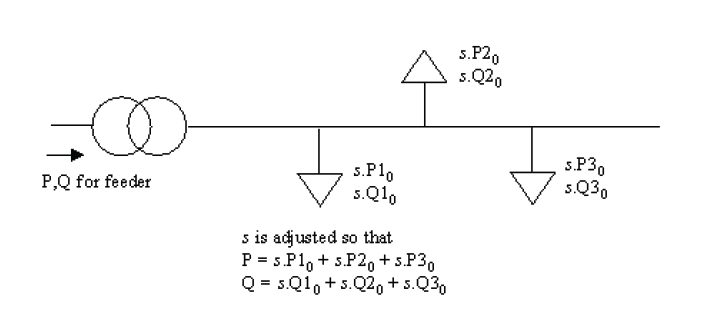
\includegraphics[width=0.9\textwidth]{images/Paper_Fig_22.png}
\setcaptionwidth{\linewidth}
\caption{负荷调节因子用以维持feeder设置的方式}
\end{figure}

以上是DIgSILENT负载潮流特性的参数介绍,对于数据的转换由于BPA只给出了负载的有功和无功所以最主要的是将有功和无功分别准确的转化DIgSILENT有功无功的输入项$P_0, Q_0$。对应的DIgsILENT数据位置如图5.7所示。

\begin{figure}[H]
\centering
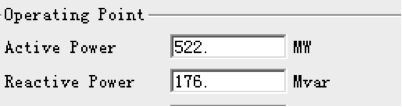
\includegraphics[width=0.6\textwidth]{images/Paper_Fig_23.png}
\setcaptionwidth{\linewidth}
\caption{负载有功,无功的转换}
\end{figure}

\subsection{DIgSILENT电抗器模型介绍及数据转换}

\begin{spacing}{1.0}
\begin{longtable}[h]{llp{0.8\columnwidth}}
\toprule
列 & 格式 & 内容\\
 \midrule
31-38 & 2F4.0 & 以MW和Mvar表示的、在基准电压下的节点并联导纳负
荷,无功:(+)=容性,(-)=感性。注意:对于BX节点,此项忽略\\
\bottomrule
\end{longtable}
\end{spacing}

R-L型电抗器:此种电抗器是电阻与电感串联构成的。为了定义电感以及电阻需要两种输入模式:

\begin{description}
\item[-] 设计参数:参数通过额定无功功率,额定电流和品质因数确定。
\item[-] 布线参数:参数通过感抗和电阻确定。
\end{description}

式5.9给出了电感L与感抗的一般关系:
$$L_{rea} = \frac{X_{rea}}{2 \pi f_{nom}} \cdot 1000 \eqno{(5.9)}$$

\begin{figure}[H]
\centering
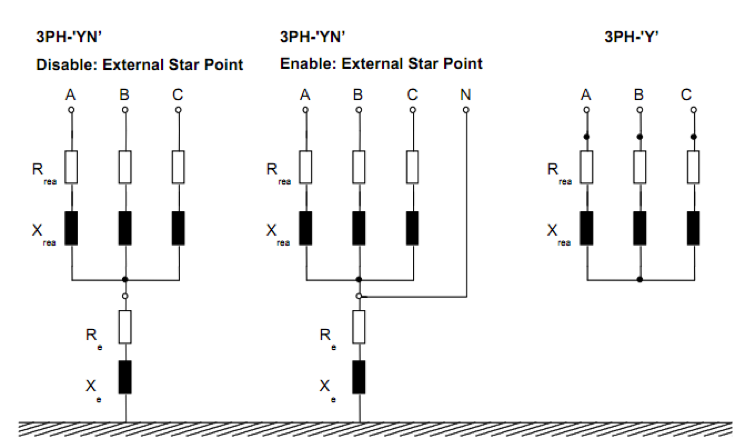
\includegraphics[width=0.9\textwidth]{images/Paper_Fig_24.png}
\setcaptionwidth{\linewidth}
\caption{\emph{3PH-'YN',3PH-'Y'}技术模型}
\end{figure}

如图5.8所示为\emph{3PH-'YN',3PH-'Y'}技术,如果内部接地阻抗星型点已经\emph{'connected'},可以将星型接法的接线点连接到中性线路(建立方式:\emph{External Star Point)}来建立\emph{'connected'}(如图2-12的二图情况)。对于中心点连接的情况,接地电阻和接地感抗需要考虑(如图2-12的一图情况),对于\emph{'disconnected'}情况,接地电阻和感抗可以忽略。

$X_{rea}, R_{rea}, Q_{rea}$的关系如式5.10和5.11所示,其中$qf_{rea}$是额定频率下的品质因数。
$$X_{rea} = \frac{U_{nom}^2}{Q_{rea}} \eqno{(5.10)}$$
$$R_{rea} = \frac{X_{nom}}{qf_{rea}} \eqno{(5.11)}$$

电抗器无功功率与额定电流关系如下:
$$Q_{rea} = \frac{I_{rea}\cdot \sqrt{3}\cdot U_{nom}}{1000} \eqno{(5.12)}$$
$$\Delta S = \Delta P + j\Delta Q = 3I^2(R + jX) = \frac{P^2 + Q^2}{U^2_j}(R + jX) \eqno{(5.13)}$$

另一种电抗器是C型电抗器:此种电抗器是纯电容型的。有两种模式可以定义C型电容器:

\begin{description}
\item[-] 设计参数:参数通过额定电容功率,额定电流。
\item[-] 布线参数:参数通过容抗和电容确定。
\end{description}

电容和电抗的关系如式5.14所示:
$$C_{rea} = \frac{B_{rea}}{2 \cdot \pi \cdot f_{rea}} \eqno{(5.14)}$$

如图5.9所示,在\emph{ABC-'YN',ABC-'Y'}技术中,如果内部接地阻抗星型点已经\emph{'connected'},可以将星型接法的接线点连接到中性线路(建立方式:\emph{External Star Point})来建立\emph{'connected'}(如图2-13的二图情况)。对于中心点连接的情况,接地电阻和接地感抗需要考虑(如图2-13的一图情况),对于\emph{'disconnected'}情况,接地电阻和感抗可以忽略。

\begin{figure}[H]
\centering
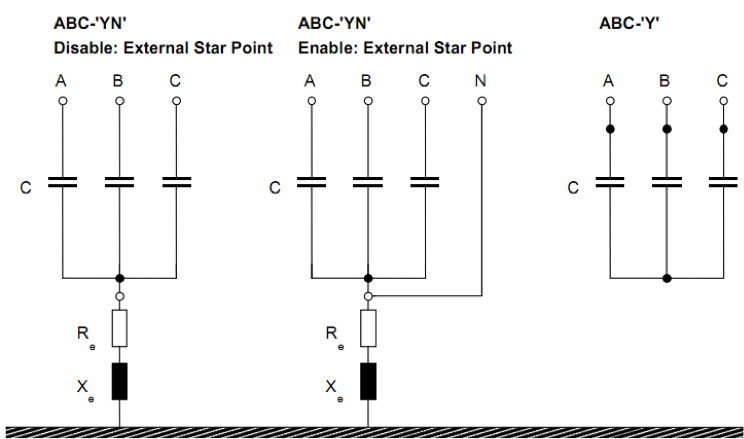
\includegraphics[width=0.9\textwidth]{images/Paper_Fig_25.png}
\setcaptionwidth{\linewidth}
\caption{\emph{ABC-'YN',ABC-'Y'}技术模型}
\end{figure}

$B_{cap}$和$Q_{cap}$的关系以及$Q_{cap}$和$I_{cap}$的关系分别如式5.15和5.16所示:
$$B_{cap} = \frac{Q_{cap}}{U_{nom}^2} \cdot 10^6 \eqno{(5.15)}$$
$$Q_{cap} = \frac{I_{cap} \cdot \sqrt{3} \cdot U_{nom}}{1000} \eqno{(5.16)}$$

R-L-C型电抗器:它由感抗,电阻,容抗串联构成。为了定义其感抗,电阻以及容抗,有两种输入模式:

\begin{description}
\item[-] a)设计参数:参数通过额定有功功率(L-C),额定电流(L-C),电感等级或共振频率或者调谐顺序以及额定频率下的品质因数或者共振频率下的品质因数。
\item[-] 布线参数:参数通过感抗或者电感,容抗或者电容大小以及电阻确定。
\end{description}

容抗$B_{cap}$和电容$C_{cap}$的关系如式5.17所示。
$$C_{cap} = \frac{B_{cap}}{2 \cdot \pi \cdot f_{nom}} \eqno{(5.17)}$$

感抗$X_{rea}$和电感$L_{rea}$的关系如式5.18所示。
$$L_{rea} = \frac{X_{rea}}{2\cdot \pi \cdot f_{nom}} \cdot 1000 \eqno{(5.18)}$$

电感等级,共振频率以及调谐顺序关系如下式所示,其中$P_{grad}$是电感度。
$$f_{res} = \frac{f_{nom}}{\sqrt{P_{grad} / 100}} \eqno{(5.19)}$$
$$n_{res} = \frac{f_{res}}{f_{nom}} \eqno{(5.20)}$$

如式5.21所示为额定频率下的品质因数与共振频率下品质因数的关系。
$$g_{reaf_{0}} = g_{rea} \cdot n_{res} = g_{rea} \cdot \frac{f_{res}}{f_{nom}} \eqno{(5.21)}$$

$g_{rea}$为额定频率下的品质因数,$g_{reaf_{0}}$为共振频率下的品质因数。

电容额定功率和额定无功功率,$L-C Q_{tot}$之间的关系如下:
$$Q_{cap} = Q_{tot} \cdot (1 - P_{grad} / 100) = Q_{tot} \cdot \left(1 - \left(\frac{f_{nom}}{f_{res}}\right)^2\right) \eqno{(5.22)}$$

$Q_{cap}$为额定电容功率,$Q_{tot}$为额定无功功率。

额定电感功率与额定无功功率,$L-C Q_{tot}$之间的关系如下:
$$Q_{cap} = Q_{tot} \cdot (100 / P_{grad} - 1) = Q_{tot} \cdot (n^2 - 1) = Q_{tot} \cdot \left(\left(\frac{f_{nom}}{f_{res}}\right)^2 - 1 \right) \eqno{(5.23)}$$

共振频率$f_{res}$由下式给出:
$$f_{res} = \frac{1}{2\pi \sqrt{L_{rea} \cdot 10^{-3} \cdot C_{cap} \cdot 10^{-6}}} \eqno{(5.24)}$$

电感,共振频率及电感之间的关系如下:
$$L_{rea} = \frac{10^3}{(2\pi f_{res}) \cdot C_{cap} \cdot 10^{-6}} \eqno{(5.25)}$$

$Q_{cap}$和$B_{cap}$之间的关系以及$X_{rea}, R_{rea}, Q_{rea}$三者之间的关系如下:
$$B_{cap} = \frac{Q_{cap}}{U_{nom}^2}\cdot 10^6 \eqno{(5.26)}$$
$$X_{rea} = \frac{U_{nom}^2}{Q_{rea}} \eqno{(5.27)}$$
$$R_{rea} = \frac{X_{rea}}{qf_{rea}} \eqno{(5.28)}$$

其中$qf_{rea}$是电阻设定为零的零的品质因数的品质因数。

以上就是对于DigSILENT中电抗器的介绍,但是上述的关键信息$qf_{rea}$在B卡中并没有给出,因此需要通过下述方法求出$qf_{rea}$。
$$I_{rea} = \frac{Q_[rea]}{\sqrt{2} \cdot U_{nom}} \cdot 1000 \eqno{(5.29)}$$
$$R_{rea} = \frac{P_{rea}}{I_{rea}^2} \cdot 1000 \eqno{(5.30)}$$
$$qf_{rea} = \frac{X_{rea}}{R_{rea}} \eqno{(5.31)}$$

而且由于B卡只提供了电抗器的无功及有功功率,无法判别其到底是R-L还是R-L-C模型,所以一般情况下只区分B卡的电抗器是C还是R-L型。(另外值得注意的是,软件中的电压都是线电压)

\subsection{DIgSILENT同步发电机模型介绍及数据转换}

\begin{spacing}{1.0}
\begin{longtable}[h]{llp{0.8\columnwidth}}
\toprule
列 & 格式 & 内容\\
 \midrule
39-42 & F4.0 & $P_{max}$:最大有功出力(MW)\\
43-47 & F5.0 & $P_{gen}$:实际有功出力(MW)\\
48-52 & F5.0 & 对于PQ节点(即B、BC、BT、BV节点)此项填所安排 的无功出力值QSCHED(Mvar);对于其它节点此项填无功出力 最大值$Q_{max}$(Mvar):(+)=容性,(-)=感性\\
53-57 & F5.0 & 无功出力最小值$Q_{min}$(Mvar)\\
58-61 & F4.3 & 所安排的电压值或者$V_{max}$(标么值)\\
62-65 & F4.3 & 所安排的$V_{min}$值(标么值),对于Vθ(即BS型)节 点,此项填角度值,注意此时省缺的格式为F4.1,单位度\\
\bottomrule
\end{longtable}
\end{spacing}

对于上面的39-65列,他们都实际上是DIgSILENT中ElmSym同步电机的数据,以下是对DIgSILENT同步电机模型的介绍。

通常情况下有两种典型的同步发电机:
\begin{description}
\item[-] 轮转子发电机以及涡轮转子发电机
\item[-] 突轴转子发电机
\end{description}

轮转子发电机模型使用在转轴以接近1500-3000转每分钟旋转。这种类型发电机通常运用于热电厂以及核电厂。转速在60到750转每分钟的低转速的同步发电机通常使用突轴转子发电机的模式,这种发电机通常使用在柴油和水能发电站。

如图5.10和5.11所示是这两种模式发电机的截面图,同时也展现了d轴和q轴的方向。

\begin{figure}[H]
\centering
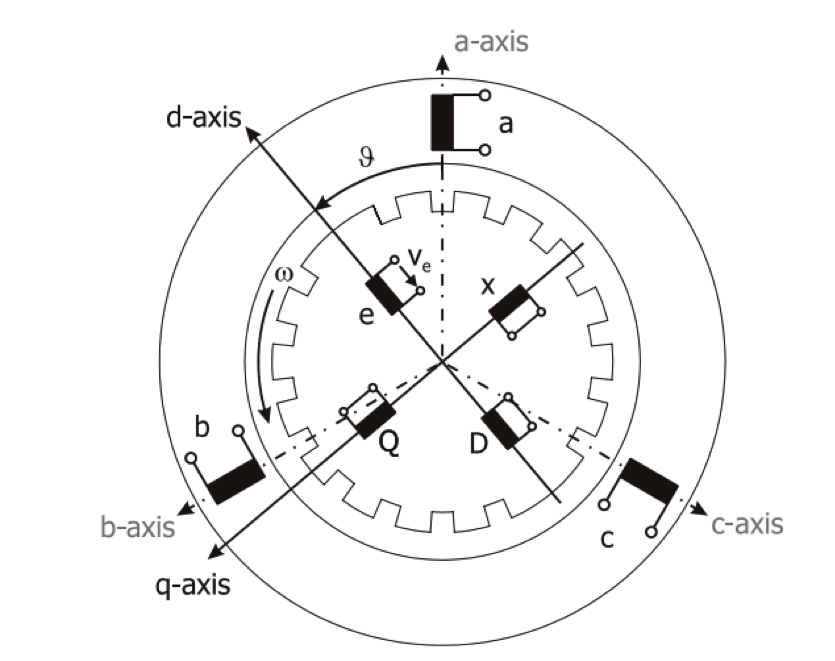
\includegraphics[width=0.7\textwidth]{images/Paper_Fig_26.png}
\setcaptionwidth{\linewidth}
\caption{轮转子同步发电机截面图}
\end{figure}

\begin{figure}[H]
\centering
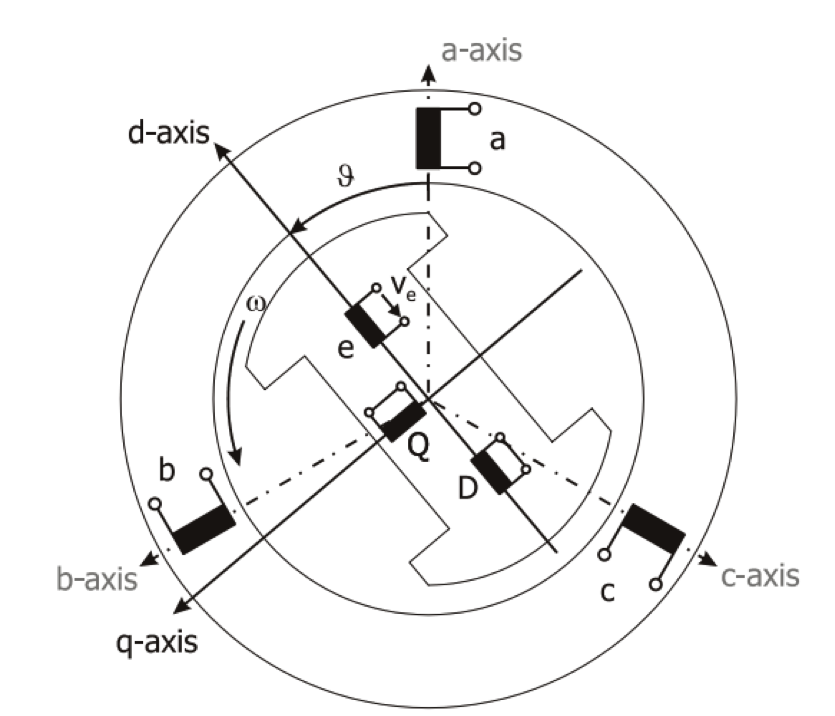
\includegraphics[width=0.6\textwidth]{images/Paper_Fig_27.png}
\setcaptionwidth{\linewidth}
\caption{突轴转子同步发电机截面图}
\end{figure}

它们分别对应于同步电机的最大用功出力,实际有功出力,最小无功出力和最大无功出力。
 
DIgSILENT中同步电机模型的建立与韩祯祥院士《电力系统分析》中介绍的一样,在此处不再赘述。建立电机特性所需要的参数如下:

\begin{table}[h]
\centering
\begin{tabular}{llll}
\toprule
DIgSILENT参数 & 对应电机参数 & 单位 & 参数范围\\
 \midrule
$tds$ & $Td$ & $'s$ & $x > 0$\\
$tqs$ & $Tq$ & $'s$ & $x\geqslant 0$\\
$tdss$ & $Td$ & $''s$ & $x > 0$\\
$tqss$ & $Tq$ & '$'s$ & $x > 0$\\
$xd$ & $xd$ & $p.u.$ & $x > 0$\\
$xds$ & $xd$ & $'p.u.$ & $x > 0$\\
$xdss$ & $xd$ & $''p.u.$ & $x > 0$\\
$xq$ & $xq$ & $p.u.$ & $x > 0$\\
$xqs$ & $xq$ & $'p.u.$ & $x \geqslant 0$\\
$xqss$ & $xq$ & $''p.u.$ & $x > 0$\\
$xdsat$ & 短路电流比 & $p.u.$ & $x \geqslant 0$\\
$xdsss$ & $xd''$ 饱和值 & $p.u.$ & $x > 0$\\
\bottomrule
\end{tabular}
\caption{同步电机建模阻抗参数}
\end{table}

图5.12展示了互感间的磁链。线性直线代表着指示需要克服气隙磁阻的励磁电流的气隙。饱和程度来源于气隙线的开环特性。

\begin{figure}[H]
\centering
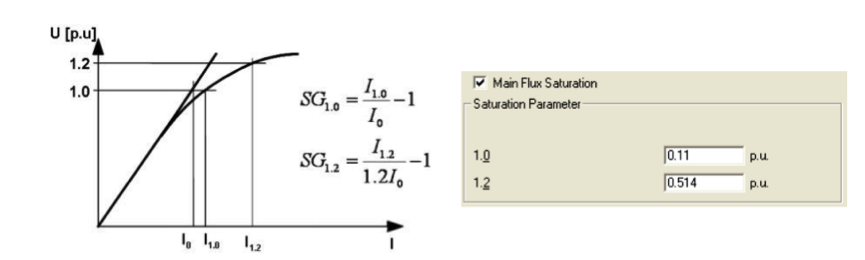
\includegraphics[width=0.9\textwidth]{images/Paper_Fig_28.png}
\setcaptionwidth{\linewidth}
\caption{开环饱和}
\end{figure}

通过指定获得无负载情况下的$1p.u$和$1.2p.u$额定发电机电压的励磁电流$I_{1.0pu}$和$I_{1.2pu}$。这样可以计算参数$s_{g1.0}(=C_{sat}(1.0pu))$和 $s_{g1.2}(=C_{sat}(1.2pu))$。

它们的计算如下:
$$s_{g1.0} = \frac{i_g(1.0p.u.)}{i_0} - 1 \eqno{(5.32)}$$
$$s_{g1.2} = \frac{i_g(1.2p.u.)}{1.2i_0} - 1 \eqno{(5.33)}$$

对于二次饱和函数:
$$A_g = \frac{1.2 - \sqrt{1.2\frac{s_{g1.2}}{s_{g1.0}}}}{1 - \sqrt{1.2\frac{s_{g1.2}}{s_{g1.0}}}} \eqno{(5.34)}$$
$$B_g = \frac{s_{g1.0}}{(1 - A_g)^2} \eqno{(5.35)}$$

以上数据主要用于暂态的计算,对于潮流计算则考虑下面几项转换数据:

BPA的B卡43-47列\emph{Pgen}项对应的就是发电机的实际有功输出及下图中DIgSILENT的\emph{Active Power}一项。

\begin{figure}[H]
\centering
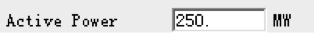
\includegraphics[width=0.4\textwidth]{images/Paper_Fig_29.png}
\setcaptionwidth{\linewidth}
\caption{实际有功转换}
\end{figure}

BPA的B卡的48~57列分别是发电机无功出力的最大与最小值,它们分别于DIgSILENT的\emph{Reactive Power Limits}中两项对应,如下图

\begin{figure}[H]
\centering
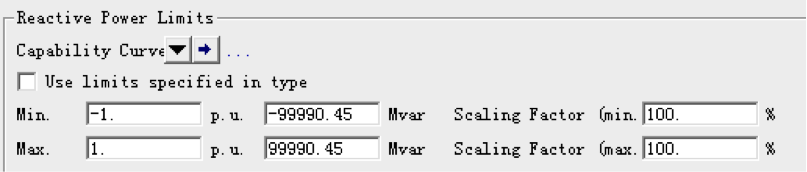
\includegraphics[width=0.7\textwidth]{images/Paper_Fig_30.png}
\setcaptionwidth{\linewidth}
\caption{无功范围转换}
\end{figure}

注意DPL中只有标幺值才能填写,只要将BPA中的有名值数据转换成标幺值填进去后,DIgSILENT会自动计算出有名值。上图中计算出来最小是-1,最大是1,那是因为改发电机的视在功率是99990.45。

对于发电机的基准功率BPA没有直接给出,在转换过程中这一项应该取BPA的基准功率。

同理B卡的39-42项则是定义发电机的最大有功出力,他对应转换的是DIgSILENT的\emph{Active Power:Operational Limits Max}一项,如下图。

\begin{figure}[H]
\centering
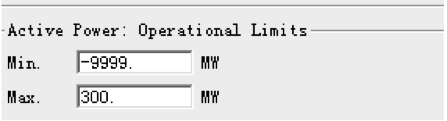
\includegraphics[width=0.5\textwidth]{images/Paper_Fig_31.png}
\setcaptionwidth{\linewidth}
\caption{有功限制}
\end{figure}

上图中\emph{Active Power:Operational Limits}中\emph{Min}一项由于BPA没有给出,一般填为-9999,这并不会影响潮流运算。

BPA的B卡58-61项则是定义了发电机的输出电压,此数据对应DIgSILENT的\emph{Dispatch}下的\emph{Voltage}一项,如下图。

\begin{figure}[H]
\centering
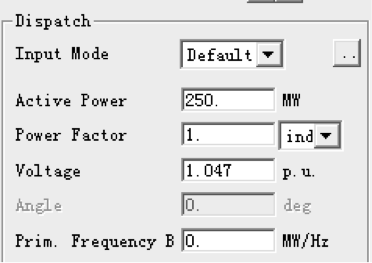
\includegraphics[width=0.4\textwidth]{images/Paper_Fig_32.png}
\setcaptionwidth{\linewidth}
\caption{发电机运行电压的转换}
\end{figure}

但是需要注意,BPA中此项数据是有名值而DIgSILENT中则是标幺值,所以需要在程序转换过程中对其数据类型进行转换。

以上即为DIgSILENT中同步发电机模型的介绍以及BPA转换为DIgSILENT数据的思路。

\begin{spacing}{1.0}
\begin{longtable}[h]{llp{0.8\columnwidth}}
\toprule
列 & 格式 & 内容\\
 \midrule
66-77 & A8,F4.0  & 对于BG和BX节点有用,填写其所要控制的节点名(66- 73)和基准电压(74-77)。要控制的电压值填在被控节点记录卡 58-61列\\
78-80 & F3.0 & 发电机在对远方节点作电压控制时,提供的无功功率的百分数\\
\bottomrule
\end{longtable}
\end{spacing}

\section{L卡,E卡}

该卡用于模拟对称的$\pi$型支路。 

在模拟母线之间连接线或者母线的常闭分段断路器时,可使用电抗值 $X=0.0001$(标么值)的一条线路。要注意的是一般情况下支路$X$之最小值取为 0.0001。

\begin{figure}[H]
\centering
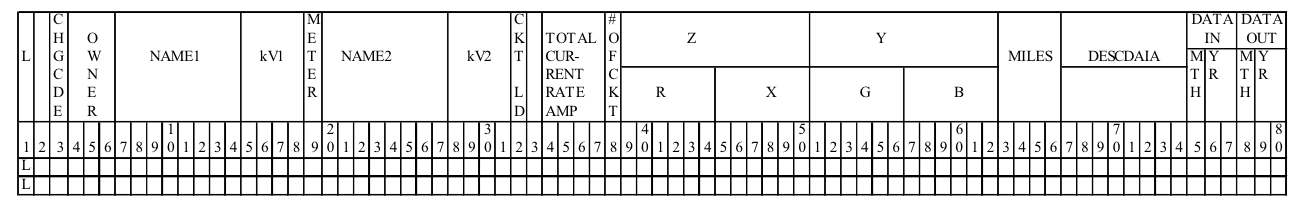
\includegraphics[width=1.05\textwidth]{images/Paper_Fig_33.png}
\setcaptionwidth{\linewidth}
\caption{L卡数据}
\end{figure}

\begin{spacing}{1.0}
\begin{longtable}[h]{llp{0.8\columnwidth}}
\toprule
列 & 格式 & 内容\\
 \midrule
1 & A1 & 卡片类型-L\\
2 & A1 & 空白\\ 
3 & A1 & 修改码 \\
4-6 & A3 & 所有者代码 \\
7-18 & A8, F4.0 & 节点名1(7-14)和基准电压(kV)(15-18) \\
19 & I1 & 区域联络线测点标记(在作区域交换功率控制时有用)\\ 
& & 填1-表示在节点1测量 \\
& & 填2-表示在节点2测量\\
& & 空白-允许程序按如下原则处理 \\
& & 1)在线路两端节点中,节点所有者与线路所有者不同
的节点为测点; \\
& & 2)当线路两端节点所有者相同时,节点1为测量点 \\
20-31  & A8, F4.0  &节点名2(20-27)和基准电压(kV)(28-31) \\
32 & A1 & 并联线路的回路标志,即回路号。 \\
34-37 &	F4.0 & 线路额定电流值,供检验线路过负荷和($N-1$)开断校
核过负荷用,单位安培 \\
38 & I1 & 并联线路数目,仅作信息用 \\
39-50&	 2F6.5 & 在系统基准电压和基准容量下的阻抗标么值:$R(39-
44),X(45-50)$ \\
51-62	& 2F6.5 & 线路对地导纳标么值(对称支路只需填一侧值):$G/2
(51-56),B/2(57-62)$。\\
63-66	& F4.1 & 线路(或段)的长度(英里),可不填 \\
67-74	& A8 & 线路说明数据(字符数字型),可不填 \\
75-77 	&A1,I2 & 投运日期:月—75列(1、2、3、4、5、6、7、8、9、
0、N、D);年号—(76-77)。可不填 \\
78-80	&A1,I2 & 停运日期,可不填\\
\bottomrule
\end{longtable}
\end{spacing}

\begin{figure}[H]
\centering
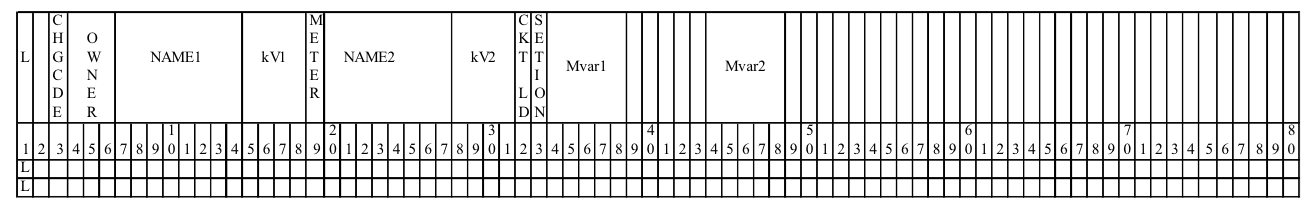
\includegraphics[width=1.05\textwidth]{images/Paper_Fig_34.png}
\setcaptionwidth{\linewidth}
\caption{E卡数据}
\end{figure}

\begin{spacing}{1.0}
\begin{longtable}[h]{llp{0.8\columnwidth}}
\toprule
列 & 格式 & 内容\\
 \midrule
1 & A1 & 卡片类型-E\\
2 & A1 & 空白\\ 
3 & A1 & 修改码 \\
4-6 & A3 & 所有者代码 \\
7-18 & A8, F4.0 & 节点名1(7-14)和基准电压(kV)(15-18) \\
19 & I1 & 在区域联络线功率控制时用的联络线测点标记,其填写规则见L卡第19列的说明\\ 
20-31  & A8, F4.0  &节点名2(20-27)和基准电压(kV)(28-31) \\
32 & A1 & 并联线路的回路标志,即回路号。 \\
34-37 &	F4.0 & 线路额定电流值,供检验线路过负荷和($N-1$)开断校
核过负荷用,单位安培 \\
38 & I1 & 并联线路数目,仅作信息用,可不填 \\
39-50&	 2F6.5 & 在系统基准电压和基准容量下的阻抗标么值:$R(39-
44),X(45-50)$ \\
51-62	& 2F6.5 & 线路对地导纳标么值(对称支路只需填一侧值):$G/2
(51-56),B/2(57-62)$。\\
63-74	& 2F6.5 & 在线路节点2端的对地导纳标么值:$G2-(63-68),B2-
(69-74) $ \\
75-77 	&A1,I2 & 投运日期:月—75列(1、2、3、4、5、6、7、8、9、
0、N、D);年号—(76-77)。可不填 \\
78-80	&A1,I2 & 停运日期,可不填\\
\bottomrule
\end{longtable}
\end{spacing}

BPA的L卡数据对应DIgSILENT里的数据类型有四种:输电线路($*.ElmLne$),电容器($*.ElmScap$),理想变压器的阻抗($*.ElmZpu$)。

这三种数据类型的区分方式:若线路两端的电压值不一致,即I端电压与J端电压不相等,则说明不是普通线路类型,需要将此元件建立为理想变压器的阻抗($*.ElmZpu$)类型。在线路电压一致的前提下,若线路的电抗值($X$)小于零,此时将元件建立为电容器模型($*.ElmScap$)。若前面两个条件皆不符合,说明是普通的输电线路,则建立输电线路模型($*.ElmLne$)。以下对DIgSILENT的这几种线路模型进行介绍。

\subsection{DIgSILENT线路模型介绍及数据转换}

\subsubsection{架空线路模型}

在DIgSILENT中,架空线路共有两种模型:

\begin{description}[1cm]
\item[1. 集总参数] 这种模型用于短传输线或者低频率下相对较长的线路中有一定的可接受精度
\item[2. 分布式参数] 由于考虑了传输线中的电波方程,这种模型比集总参数模型更加精确,它用于长线以及高频线路模型中
\end{description}

下面就对这两种参数做进一步介绍。

\begin{figure}[H]
\centering
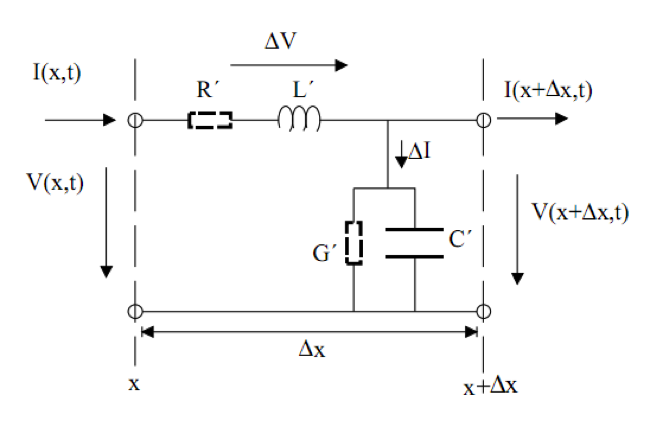
\includegraphics[width=0.9\textwidth]{images/Paper_Fig_35.png}
\setcaptionwidth{\linewidth}
\caption{DIgSILENT线路模型}
\end{figure}

依靠这个模型可以推导出下面的分布式和集总式两种简化模型,而推导过程需要的参数就是上图中的$R', Z', B', G'$。

如图5.20所示,线路模型的参数实际上都是依赖于此模型经行推导的。

其中:
$$Z_{\pi} = Z_c \cdot sinh\gamma \cdot l = Z' \cdot l \cdot \frac{sinh\gamma \cdot l}{\gamma \cdot l} \eqno{(5.36)}$$
$$Y_{\pi} = \frac{cosh\gamma \cdot l - 1}{Z_c \cdot sinh\gamma \cdot l} = \frac{1}{2} \cdot {\gamma}' \cdot l \cdot \frac{thg\left(\frac{\gamma \cdot l}{2}\right)}{\frac{\gamma \cdot l}{2}} \eqno{(5.37)}$$

$\gamma$是传播系数$\gamma = \sqrt{Z' \cdot \gamma'}$。

$Z'$和$Y'$是单位长度等值阻抗和导纳。

图5.20中的$Z_{\pi}$和$Y_{\pi}$是频率依赖参数。

使用分布参数模型需要在\emph{ElmLne}的\emph{basic page}中选定\emph{“Distributed Parameter”},如下图:

\begin{figure}[H]
\centering
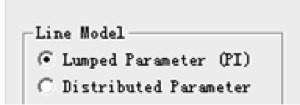
\includegraphics[width=0.4\textwidth]{images/Paper_Fig_36.png}
\setcaptionwidth{\linewidth}
\caption{分布参数模型的选择}
\end{figure}

集总式分布参数模型表达式如下:
$$Z_{\pi} = B = Z' \cdot l = R' \cdot l + j\omega \cdot L' \cdot l \eqno{(5.38)}$$
$$Y_{\pi} = \frac{A - 1}{B} = \frac{1+\frac{1}{2}\cdot Z' \cdot Y' \cdot l^2}{Z' \cdot l} = \frac{1}{2} \cdot Y' \cdot l = \frac{1}{2} \cdot (G' \cdot l + j\omega \cdot C' \cdot l) \eqno{(5.39)} $$

电路模型图如下图。与分布式参数模型不同,这个模型有离散$R,L,G$以及$C$。因此此模型不仅适用于稳定状态计算也可以用于暂态仿真计算。

\begin{figure}[H]
\centering
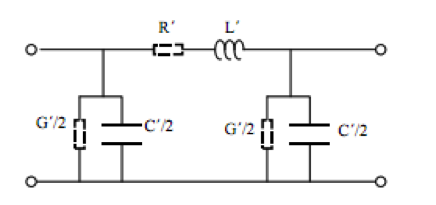
\includegraphics[width=0.7\textwidth]{images/Paper_Fig_37.png}
\setcaptionwidth{\linewidth}
\caption{传输线集总模型}
\end{figure}

使用集总参数模型需要在\emph{ElmLne}的\emph{basic page}中选定\emph{“Lumped Parameter”}如下图:

\begin{figure}[H]
\centering
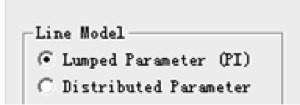
\includegraphics[width=0.4\textwidth]{images/Paper_Fig_38.png}
\setcaptionwidth{\linewidth}
\caption{集总参数模型的选择}
\end{figure}

模型的精准性依赖于因子$f \cdot l$。对于架空线在小于250km以及电力系统频率下,等效是很有效的,其产生的误差可以忽略。

对于BPA到DIgSILENT数据的转换过程中,BPA提供的是的$\pi$模型参数$X,R,B,G$,所以需要逆推导图5.19中的 。但是以DIgSILENT的DPL提供的运算功能,实现这个逆推导的过程基本不可行,而且由于BPA中还存在有不对称电路,此时是无法等效为$\pi$模型电路的,因此我换了一种方法处理这个问题。

下图中的 部分实际上可以看为一个电容与电阻的并联,这正好与DIgSILENT的SHUNT元件的C型电抗相似,所以可以用两个C型电抗去代替$Y\pi$,而线路只需要知道其单位阻抗$Z'$,线路的$B', G'$直接填为0。下面我会证明$Z'$可以使用BPA中$X,R$求出的阻抗去替换。

证明:
$$Z = \frac{sinh\gamma l}{\gamma l}Z'l \eqno{(5.40)}$$

由于$l$一般取1,所以上式又可写为:
$$Z = \frac{sinh\gamma}{\gamma}Z'l \eqno{(5.41)}$$
$$\gamma = \sqrt{Z' \cdot Y'}$$

由于计算处理过程$B', G'$实际上是给$B', G'$赋予一个无穷趋于0的值,所以可以看为$\gamma \rightarrow 0$。

由级数展开:
$$sinh\gamma l = \gamma l + \frac{(\gamma l)^3}{3!} + \frac{(\gamma l)^5}{5!} + \frac{(\gamma l)^7}{7!} + ... \eqno{(5.43)}$$
$$\lim\limits_{\gamma\to0}\frac{sinh\gamma}{\gamma} = \lim\limits_{\gamma\to0}\frac{\gamma + \frac{(\gamma)^3}{3!} + \frac{(\gamma)^5}{5!} + \frac{(\gamma)^7}{7!} + ...}{\gamma} = 1 \eqno{(5.44)}$$

所以可得
$$Z = Z'$$

这样,可以直接用BPA求出的$Z$去替换DIgSILENT线路参数中的$Z'$。

DIgSILENT中C型电抗的模型如图5.23:

\begin{figure}[H]
\centering
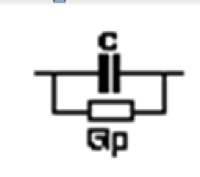
\includegraphics[width=0.2\textwidth]{images/Paper_Fig_39.png}
\setcaptionwidth{\linewidth}
\caption{DIgSILENT中C型电抗的模型}
\end{figure}

而现在知道BPA中的$Y\pi$参数,而DIgSILENT中C型电抗的模型参数则是有其电容和电阻上的有功与无功推导的,所以这里需要经行一个逆推导,过程如下:
$$Q_c = YB \cdot U_B^2 \eqno{(5.46)}$$
$$P_r = YG \cdot U_B^2 \eqno{(5.47)}$$

通过上述模型的建立就可以完成DIgSILENT对BPA中对称电路与不对称电路的转换建模了。

DIgSILENT中电容器模型如图5.24所示。

\begin{figure}[H]
\centering
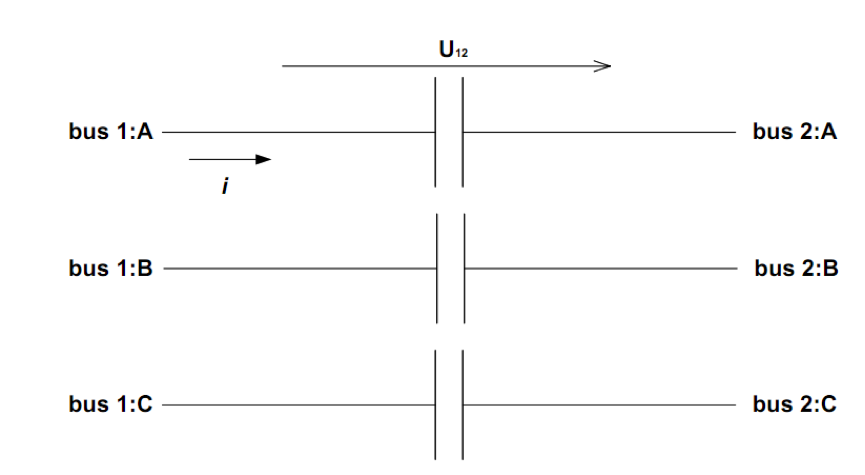
\includegraphics[width=0.6\textwidth]{images/Paper_Fig_40.png}
\setcaptionwidth{\linewidth}
\caption{DIgSILENT中电容器模型}
\end{figure}

交流模型中
$$I = j\omega_{\pi}CU \eqno{(5.48)}$$

直流模型中,由于纯电容是隔直流的,所以模型可以看为一无穷大电阻,即
$$I = 0 \eqno{(5.49)}$$

变压器的阻抗模型中,包含理想变压器的感抗模型。
\begin{figure}[H]
\centering
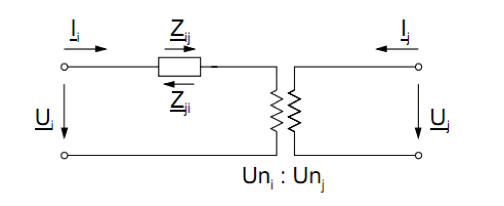
\includegraphics[width=0.6\textwidth]{images/Paper_Fig_41.png}
\setcaptionwidth{\linewidth}
\caption{ 公共阻抗正,负,零序绝对值模型}
\end{figure}

\begin{figure}[H]
\centering
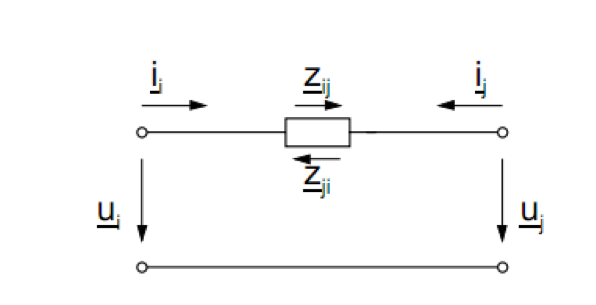
\includegraphics[width=0.6\textwidth]{images/Paper_Fig_42.png}
\setcaptionwidth{\linewidth}
\caption{公共阻抗正,负,零序标幺值模型}
\end{figure}

此模型在潮流分析需要注意的参数如下表:

\begin{table}[h]
\centering
\begin{tabular}{lll}
\toprule
DIgSILENT参数 & 对应电机参数 & 单位\\
 \midrule
Sn & 额定功率 & MVA\\
nphase & 相数(三相或一相模型) & 1或3\\
iequalz & 等阻抗$z_{ij} = z_{ji}$ & 使能/不使能\\
r\_pu, x\_pu & $'i-j'$正序阻抗 & $p.u.$\\
r\_pu\_ji, x\_pu\_ji & $'j-i'$正序阻抗 & $p.u.$ \\
r0\_pu, x0\_pu & $'i-j'$零序阻抗 & $'p.u.$ \\
r0\_pu\_ji, x0\_pu\_ji & $'j-i'$零序阻抗 & $''p.u.$ \\
iz2eqz1 & 阻抗$z_2 = z_1$ & 使能/不使能 \\
r2\_pu, x2\_pu & $'i-j'$负序阻抗 & $'p.u.$\\
r2\_pu\_ji, x2\_pu\_ji & $'j-i'$负序阻抗 & $''p.u.$\\
\bottomrule
\end{tabular}
\caption{公共阻抗输入参数}
\end{table}

\subsubsection{线路数据转换}

线路的名称是以BPA线路两端节点名命名。

比如在039BPA数据中,BUS-10与BUS-11之间的线路则命名为\emph{lne\_BUS-11\_BUS-12\_1},其中最后一位数字1是用于区别是否这两个节点有并联母线的,转换如下图:

\begin{figure}[H]
\centering
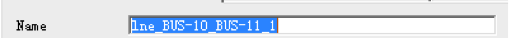
\includegraphics[width=0.6\textwidth]{images/Paper_Fig_43.png}
\setcaptionwidth{\linewidth}
\caption{线路数据转换}
\end{figure}

正如前面对BPA的L卡介绍中提到的第19项数据METER用于判断基准节点。在转换过程中我也是通过此项选择基准节点的,而选择的思想就如L卡中对METER功能介绍的方法一样。

对于线路的长度则参照BPA中数据转换,如果BPA数据没填,则DIgSILENT中使用默认的1km,转换如下图:

\begin{figure}[H]
\centering
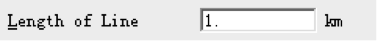
\includegraphics[width=0.6\textwidth]{images/Paper_Fig_44.png}
\setcaptionwidth{\linewidth}
\caption{线路长度}
\end{figure}

在建立好输电线路模型(\emph{*.ElmLne})以后,由于DIgSILENT对这种数据的储存用了两个数据块,所以需要建立它的Type文件,输电线路类型(\emph{*.TypLne}),这两个文件同时储存一条输电线路的数据。

在\emph{TypLne}中额定电流就是指定参考节点的电压,额定电流就是L卡中额定电流一项数据卡数据。

在数据转换过程中,需要注意的是DIgSILENT采用的是有名值,BPA采用的是标幺值。需要进行转换。有名值与标幺值之间的转换公式为(其中有上标的为有名值):
$$R = R' \cdot l \cdot \frac{100}{U^2_R}, X = X' \cdot l \cdot \frac{100}{U^2_N}, B = B' \cdot l \cdot \frac{U_N^2}{100} \eqno{(5.50)}$$

由于正序网络结构的各元件参数与正常运行的等值网络相同。因此只需要将元件转换好的有名电阻直接转换到上述正负序项中即可。

\subsection{L+卡}

\begin{figure}[H]
\centering
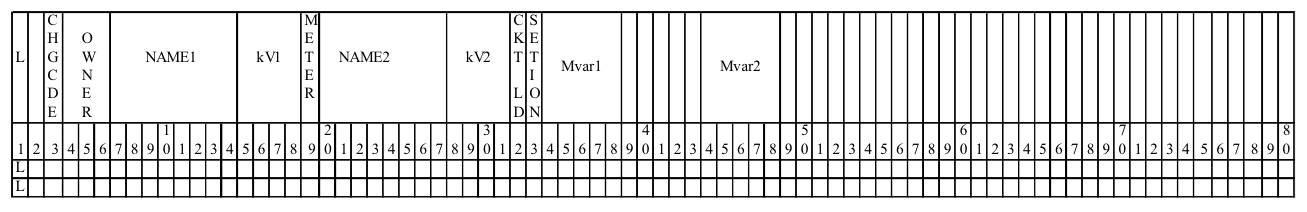
\includegraphics[width=1.05\textwidth]{images/Paper_Fig_45.png}
\setcaptionwidth{\linewidth}
\caption{L+卡数据}
\end{figure}

\begin{spacing}{1.0}
\begin{longtable}[h]{llp{0.8\columnwidth}}
\toprule
列 & 格式 & 内容\\
 \midrule
1 & A1 & 卡片类型-L\\
2 & A1 & 空白\\ 
3 & A1 & 修改码 \\
4-6 & A3 & 所有者代码 \\
7-18 & A8, F4.0 & 节点名1(7-14)和基准电压(kV)(15-18) \\
20-31& A8, F4.0 & 节点名2(20-27)和基准电压(kV)(28-31)\\ 
32 & A1 & 并联线路的回路标志,即回路号。 \\
34-38 &F5.0 & 线路前侧高抗容量(Mvar,填正值) \\
44-48 &F5.0 & 线路后侧高抗容量(Mvar,填正值)\\
\bottomrule
\end{longtable}
\end{spacing}

我国电力系统正在向大容量、远距离、超(特)高的方向发展。超高压输电压系统由于其电压等级提高,可传输更大的容量,更远的距离,但是线路的电容效应限制了传输容量,降低了系统静态和动态稳性,增加了工频过电压幅值,所以超高压输电线路往装设并联高压电抗器(下文简称高抗)解决无功平衡和过电压问题。

而L+卡的目的实际上就是为了模拟超高电压下的电抗器,起到抵消电容效应的作用。而DIgSILENT电抗器在前文有详细介绍,这里就不赘述了。

\subsection{T卡}

